\documentclass[11pt]{article}
\usepackage[left= 1.55cm, right = 1.55cm,top = 1.2cm, bottom = 1.5cm]{geometry}
\usepackage{enumerate}
\usepackage{amsmath,amsfonts,amssymb}
\usepackage{setspace}
\usepackage{float}
\usepackage{multicol}
\usepackage{xcolor}
\usepackage[hidelinks]{hyperref}
\usepackage{listings}
\definecolor{codegreen}{rgb}{0,0.6,0}
\definecolor{codegray}{rgb}{0.5,0.5,0.5}
\definecolor{codepurple}{rgb}{0.58,0,0.82}
\definecolor{backcolour}{rgb}{0.95,0.95,0.92}
\lstdefinestyle{mystyle}{
    backgroundcolor=\color{backcolour},   
    commentstyle=\color{codegreen},
    keywordstyle=\color{magenta},
    numberstyle=\tiny\color{codegray},
    stringstyle=\color{codepurple},
    basicstyle=\ttfamily\footnotesize,
    breakatwhitespace=false,         
    breaklines=true,                 
    captionpos=b,                    
    keepspaces=true,                 
    numbers=left,                    
    numbersep=5pt,                  
    showspaces=false,                
    showstringspaces=false,
    showtabs=false,                  
    tabsize=2
}
\lstset{style=mystyle}
\pagenumbering{gobble}
\renewcommand{\arraystretch}{1.5}
\usepackage{mathtools}
\usepackage{longtable}
\usepackage{graphicx}
\usepackage{multirow}
\usepackage{hhline}
\usepackage[utf8]{inputenc}
\usepackage[usestackEOL]{stackengine}
\setlength{\abovedisplayskip}{0in}
\setlength{\columnsep}{3em}
\newcommand{\blue}{\color{Blue}}
\newcommand{\green}{\color{Green}}
\usepackage[inkscapeformat=png]{svg}
\newcommand{\red}{\color{Red}}
\newcommand{\black}{\color{Black}}
\newcommand{\Name}{Communities }
\title{Software Requirements Analysis\\\Name : A Social Media Platform\\ SM02}
\author{Harshit Pant \\ CS21BTECH11021 \and Satpute Aniket Tukaram \\ CS21BTECH11056 \and Mahin Bansal \\ CS21BTECH11034 \and Burra Vishal Mathews \\ CS21BTECH11010}
\date{}
\begin{document}
\maketitle
\begin{center}
    \tableofcontents
\end{center}
\section{Context Diagram}
\begin{figure}[H]
    \centering
    \makebox[\linewidth][c]{\hspace{5cm}
        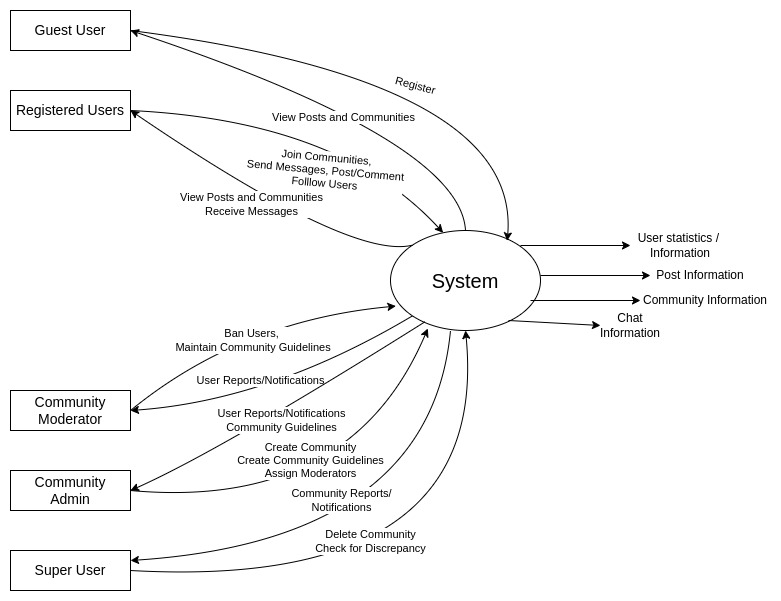
\includegraphics[width = 0.8\textwidth]{./images/context_diagram.jpeg}
    }
    \caption{Context Diagram}
    \label{fig:context_diagram}
\end{figure}
\newpage
\section{Data Flow Diagrams}
\subsection{DFD Descriptions}
Below are two possible DFDs for the system.

\begin{figure}[H]
    \centering
    \makebox[\linewidth][c]{
        \includegraphics[width = 0.8\textwidth]{./images/dfd_wrong.png}
    }
    \caption{Incorrect DFD}
\end{figure}
\begin{itemize}
    \item The red line marks the man-machine boundary in the DFD design.
\end{itemize}
\newpage
\begin{figure}[H]
    \centering
    \makebox[\linewidth][c]{\hspace{1cm}
        \includegraphics[width = \textwidth]{./images/dfd_correct.png}
    }
    \caption{Correct DFD}
\end{figure}

\begin{itemize}
    \item The red line marks the man-machine boundary in the DFD design.
\end{itemize}
\newpage
\subsection{Comparing the two DFDs}
\newpage
\section{Function Point Analysis}
\begin{table}[H]
    \centering
    \begin{tabular}{|p{3cm}|p{3cm}|p{3cm}|p{3cm}|}
        \hline
        \textbf{Function Type}  & \textbf{Simple} & \textbf{Medium} & \textbf{Complex} \\
        \hline
        External Input          & 3               & 4               & 6                \\
        \hline
        External Output         & 4               & 5               & 7                \\
        \hline
        External Inquiry        & 3               & 4               & 6                \\
        \hline
        Internal Logical File   & 7               & 10              & 15               \\
        \hline
        External Interface File & 5               & 7               & 10               \\
        \hline
    \end{tabular}
    \caption{Function Point Complexity Weights}
\end{table}

\subsection{UFP Caluculation}

\begin{itemize}
    \item \textbf{External Input:} Data or control information that comes from outside the application's boundary.
    \item \textbf{External Output:} Data or control information that is sent to outside the application's boundary.
    \item \textbf{External Inquiry:} Input-output combination, where input causes and immediate output and leaves the data intact.
    \item \textbf{Internal Logical File:} A user identifiable group of logically related data that resides entirely within the application boundary and is maintained through external inputs.
    \item \textbf{External Interface File:} A user identifiable group of logically related data that is used for reference purposes only.
\end{itemize}

Now we need to count the number of each of these in our system.\\

\begin{itemize}
    \item \textbf{External Input:}
          \begin{enumerate}
              \item
          \end{enumerate}
\end{itemize}
\end{document}